\chapter{Binomial and Geometric Distributions}\index{binomial distribution}\index{geometric distribution}

Your school's best free-throw shooter makes 70\% of their shots. In tonight's game,
they will probably shoot about 10. What are the chances they make exactly 7? At
least 8? And a different question: a pack of trading cards has a 1-in-8 chance of
holding a rare card. How many packs will you probably have to open before you get
one?

The first question counts \emph{successes in a fixed number of tries}. The second
counts \emph{tries until the first success}. These two patterns show up everywhere:
free throws and penalty kicks, defective parts on an assembly line, patients who
respond to a medicine, days until a rainy day. Each has its own probability
distribution, and both are on the AP Statistics exam.

\section{The Binomial Setting}\index{binomial setting}
A random variable $X$ has a \newterm{binomial distribution} when it counts the
number of successes in a situation that meets four conditions. A handy way to
remember them is \textbf{BINS}:
\begin{itemize}
\item \textbf{B}inary: each trial has two outcomes, success or failure.
\item \textbf{I}ndependent: the result of one trial does not change the chances for another.
\item \textbf{N}umber: the number of trials, $n$, is fixed in advance.
\item \textbf{S}ame probability: every trial has the same chance of success, $p$.
\end{itemize}
Ten free throws by a 70\% shooter fit: each shot goes in or not, one shot does not
affect the next (we assume), there are 10 shots, and each has $p = 0.7$. So the
number made, $X$, is binomial with $n = 10$ and $p = 0.7$.

\subsection{The Binomial Formula}
What is the chance of making exactly 7 of the 10? One way is
$$\text{make, make, make, make, make, make, make, miss, miss, miss}$$
By independence, its probability is $0.7^7 \cdot 0.3^3$. But the 3 misses could
come at any 3 of the 10 shots, and every arrangement has the same probability.
The number of arrangements is the number of ways to choose which 7 shots go in,
$\binom{10}{7} = 120$, from the Discrete Probability and Counting chapter. So
$$P(X = 7) = \binom{10}{7}(0.7)^7(0.3)^3 = 120(0.0823543)(0.027) \approx 0.2668$$

\begin{mdframed}[style = important, frametitle = {The Binomial Distribution}]
If $X$ counts the successes in $n$ independent trials, each with success probability
$p$, then for $k = 0, 1, \dots, n$,
$$P(X = k) = \binom{n}{k}p^k(1 - p)^{n - k}$$
\end{mdframed}

Each piece has a job: $p^k$ for the $k$ successes, $(1 - p)^{n - k}$ for the
$n - k$ failures, and $\binom{n}{k}$ for all the orders they could come in.

\begin{figure}[H]
\centering
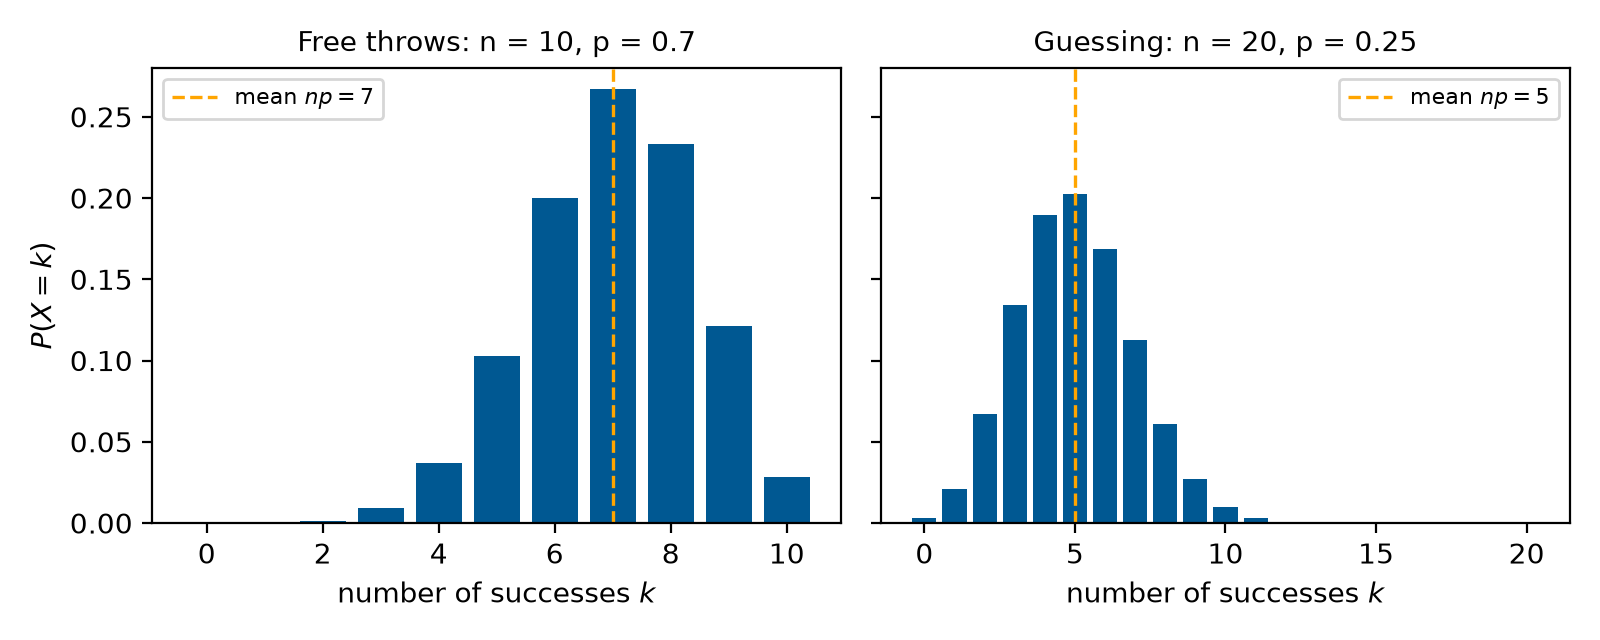
\includegraphics[width=0.95\textwidth]{binomial_pmfs.png}
\caption{Two binomial distributions. Left: a 70\% shooter taking 10 free throws.
Right: guessing on 20 multiple-choice questions with 4 choices each.}
\label{fig:binomial-pmfs}
\end{figure}

\subsection{``At Least'' and ``At Most''}
Most real questions ask about a range. The chance of making at least 8 is the sum of
three cases:
$$P(X \geq 8) = P(X = 8) + P(X = 9) + P(X = 10) \approx 0.2335 + 0.1211 + 0.0282 = 0.3828$$
When a range has many terms, use the \textbf{complement}. For example, the chance
of making at least 1 shot is $1 - P(X = 0) = 1 - 0.3^{10}$, which is extremely close
to 1. On AP-style problems, read the wording carefully: ``at least 8'' includes 8,
while ``more than 8'' does not.

\subsection{Mean and Standard Deviation}\index{binomial distribution!mean and standard deviation}
Here is a slick way to find the mean. Think of $X$ as a sum of $n$ simple random
variables, one per trial: $X_i = 1$ if trial $i$ succeeds and $0$ if it fails. Each
$X_i$ has
$$E[X_i] = 1 \cdot p + 0 \cdot (1 - p) = p, \qquad \operatorname{Var}(X_i) = E[X_i^2] - p^2 = p - p^2 = p(1 - p)$$
By linearity of expectation (from the Random Variables chapter), and because
variances of independent variables add,

\begin{mdframed}[style = important, frametitle = {Binomial Mean and Standard Deviation}]
$$\mu = np, \qquad \sigma = \sqrt{np(1 - p)}$$
\end{mdframed}

The 70\% shooter taking 10 shots averages $\mu = 10(0.7) = 7$ makes, with standard
deviation $\sqrt{10(0.7)(0.3)} = \sqrt{2.1} \approx 1.45$. A night with 5 makes is
unremarkable; a night with 2 would be very unusual.

\subsection{Shape}
Look again at figure \ref{fig:binomial-pmfs}. When $p$ is close to $\frac{1}{2}$, the
distribution is nearly symmetric. When $p$ is near 0 or 1, it piles up at one end
and has a tail on the other side (the free-throw distribution is skewed left). As $n$
grows, the shape becomes more and more bell-shaped. A common rule: if both
$np \geq 10$ and $n(1 - p) \geq 10$, the binomial distribution is close to a normal
distribution. You will use that fact constantly in the inference chapters of
Volume 30.

\subsection{Sampling Without Replacement: The 10\% Condition}\index{10\% condition}
When you survey people, you never ask the same person twice, so the trials are not
quite independent. If 15\% of a school's 2,000 students are left-handed and you pick
25 at random, finding a lefty slightly lowers the chance that the next person is one.
But the effect is tiny when the sample is small compared with the population. The
\newterm{10\% condition} says: if the sample is no more than 10\% of the population,
you can treat the count as binomial anyway. Here, 25 is far less than 200, so a
binomial model is fine.

\section{Binomial Probabilities in Python}
Calculators have \texttt{binompdf} and \texttt{binomcdf} functions. In Python, the SciPy
library's \texttt{stats} module has \texttt{binom} (and \texttt{geom}, for the next
section). The \texttt{pmf} function gives $P(X = k)$, \texttt{cdf} gives
$P(X \leq k)$, and \texttt{sf} (for ``survival function'') gives $P(X > k)$.

\begin{minted}{python}
from scipy.stats import binom, geom

# Free throws: n = 10 shots, p = 0.7
print(round(binom.pmf(7, 10, 0.7), 4))      # P(X = 7)
print(round(binom.sf(7, 10, 0.7), 4))       # P(X > 7), that is, P(X >= 8)
print(binom.mean(10, 0.7), round(binom.std(10, 0.7), 3))

# Rare cards: p = 1/8 per pack
print(round(geom.pmf(3, 0.125), 4))         # first rare card in pack 3
print(round(geom.sf(10, 0.125), 4))         # P(X > 10): none in 10 packs
print(geom.mean(0.125), round(geom.std(0.125), 2))
\end{minted}
\begin{verbatim}
0.2668
0.3828
7.0 1.449
0.0957
0.2631
8.0 7.48
\end{verbatim}

You can also check a formula by simulation, as in the Monte Carlo Simulation chapter.
Here are 100,000 nights of 10 free throws each:
\begin{minted}{python}
import random

random.seed(10)

trials = 100_000
exactly_7 = 0
for _ in range(trials):
    made = sum(random.random() < 0.7 for _ in range(10))   # 10 shots
    if made == 7:
        exactly_7 += 1
print(exactly_7 / trials)
\end{minted}
\begin{verbatim}
0.26648
\end{verbatim}
The simulation agrees with the formula's $0.2668$ to about three decimal places.

\begin{Exercise}[title={Is It Binomial?}, label=bg_bins]
For each random variable, decide whether it has a binomial distribution. If not, say
which BINS condition fails.
\begin{enumerate}
\item The number of sixes in 10 rolls of a fair die.
\item The number of cards you draw from a shuffled deck until you get an ace.
\item The number of hearts in 5 cards dealt from a shuffled deck.
\item The number of days next week on which it rains, if rainy days tend to come in streaks.
\end{enumerate}
\end{Exercise}
\begin{Answer}[ref=bg_bins]
\begin{enumerate}
\item Binomial, with $n = 10$ and $p = \frac{1}{6}$.
\item Not binomial: the number of trials is not fixed. (If cards were replaced and
reshuffled each time, this would be geometric.)
\item Not exactly binomial: the cards are drawn without replacement, so the trials are
not independent. But 5 cards is less than 10\% of 52 (5.2), so a binomial model with
$n = 5$ and $p = \frac{1}{4}$ is a reasonable approximation.
\item Not binomial: streaks mean the days are not independent.
\end{enumerate}
\end{Answer}

\begin{Exercise}[title={Lefties}, label=bg_lefty]
About 15\% of people are left-handed. In a random group of 25 students:
\begin{enumerate}
\item What is the probability that exactly 3 are left-handed?
\item What is the probability that at least one is left-handed?
\item Find the mean and standard deviation of the number of lefties.
\end{enumerate}
\end{Exercise}
\begin{Answer}[ref=bg_lefty]
\begin{enumerate}
\item $\binom{25}{3}(0.15)^3(0.85)^{22} \approx 0.217$.
\item $1 - P(X = 0) = 1 - 0.85^{25} \approx 0.983$.
\item $\mu = 25(0.15) = 3.75$ and $\sigma = \sqrt{25(0.15)(0.85)} \approx 1.79$.
\end{enumerate}
\end{Answer}

\begin{Exercise}[title={Just Guessing}, label=bg_guess]
A quiz has 20 multiple-choice questions with 4 choices each. A student guesses on every
question.
\begin{enumerate}
\item What are the mean and standard deviation of the number correct?
\item Use Python to find the probability of getting 5 or fewer right, and the probability
of getting at least 12 right (a passing grade).
\end{enumerate}
\end{Exercise}
\begin{Answer}[ref=bg_guess]
\begin{enumerate}
\item $\mu = 20(0.25) = 5$ and $\sigma = \sqrt{20(0.25)(0.75)} \approx 1.94$.
\item \mintinline{python}{binom.cdf(5, 20, 0.25)} gives $P(X \leq 5) \approx 0.617$, and
\mintinline{python}{binom.sf(11, 20, 0.25)} gives $P(X \geq 12) \approx 0.0009$. Guessing
passes less than one time in a thousand.
\end{enumerate}
\end{Answer}

\section{The Geometric Setting}\index{geometric setting}
Now change the question. Instead of fixing the number of trials and counting
successes, keep going \emph{until the first success}, and count the trials. If the trials
are binary and independent with the same success probability $p$, the number of the
trial on which the first success happens, $X$, has a \newterm{geometric distribution}.

For the first success to come on trial $k$, the first $k - 1$ trials must all fail, and
then trial $k$ must succeed. There is only one way for that to happen, so no binomial
coefficient is needed:

\begin{mdframed}[style = important, frametitle = {The Geometric Distribution}]
If $X$ is the trial on which the first success occurs, then for $k = 1, 2, 3, \dots$,
$$P(X = k) = (1 - p)^{k - 1}p$$
and the chance of needing more than $k$ trials is
$$P(X > k) = (1 - p)^k$$
\end{mdframed}

The second formula holds because needing more than $k$ trials means the first $k$ all
failed.

\textbf{Example}: Each pack of cards has a rare card with probability $p = \frac{1}{8}$.
\begin{itemize}
\item The chance that the first rare card is in the 3rd pack is
$\left(\frac{7}{8}\right)^2\frac{1}{8} \approx 0.0957$.
\item The chance that you open 10 packs and still have no rare card is
$\left(\frac{7}{8}\right)^{10} \approx 0.263$. More than a quarter of collectors will be
that unlucky.
\end{itemize}

\begin{figure}[H]
\centering
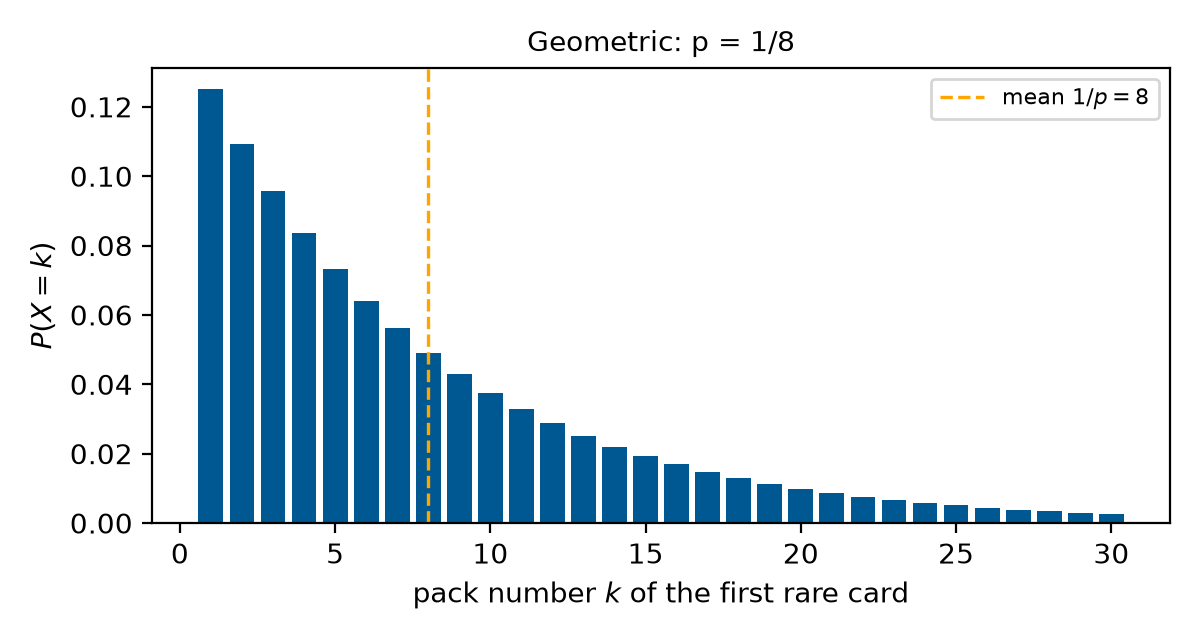
\includegraphics[width=0.7\textwidth]{geometric_pmf.png}
\caption{The geometric distribution with $p = \frac{1}{8}$. Each bar is $\frac{7}{8}$ as tall
as the one before it, so the most likely single outcome is always $k = 1$.}
\label{fig:geometric-pmf}
\end{figure}

\subsection{Mean and Standard Deviation}\index{geometric distribution!mean}
How many packs should you expect to open? There is a neat argument. Let $\mu$ be the
expected number of trials. You always open the first pack. With probability $1 - p$, it
has no rare card, and then you are back where you started, needing $\mu$ more packs
on average. So
$$\mu = 1 + (1 - p)\mu \quad\Longrightarrow\quad p\mu = 1 \quad\Longrightarrow\quad \mu = \frac{1}{p}$$

\begin{mdframed}[style = important, frametitle = {Geometric Mean and Standard Deviation}]
$$\mu = \frac{1}{p}, \qquad \sigma = \frac{\sqrt{1 - p}}{p}$$
\end{mdframed}

With $p = \frac{1}{8}$, you expect to open $8$ packs, which matches common sense: a
1-in-8 event takes 8 tries on average. The standard deviation is
$\frac{\sqrt{7/8}}{1/8} \approx 7.48$, almost as large as the mean. Geometric waits are
very unpredictable: you might get lucky on the first pack or wait 25.

\subsection{No Memory}\index{memoryless property!geometric}
Suppose you have already opened 10 packs with no rare card. Are you ``due''? No. The
packs are independent, so the chance of needing more than 5 \emph{additional} packs is
$\left(\frac{7}{8}\right)^5$, exactly the same as for someone just starting. The geometric
distribution is \newterm{memoryless}: the past does not change the future. Believing
otherwise is called the \newterm{gambler's fallacy}. The next chapter's exponential
distribution, which models waiting times in continuous time, has the same property.

\begin{Exercise}[title={The First Miss}, label=bg_miss]
The 70\% free-throw shooter keeps shooting until they miss.
\begin{enumerate}
\item What is the probability that their first miss is on their 4th shot?
\item How many shots should they expect to take, including the miss?
\end{enumerate}
\end{Exercise}
\begin{Answer}[ref=bg_miss]
Here a ``success'' is a miss, with $p = 0.3$.
\begin{enumerate}
\item $(0.7)^3(0.3) \approx 0.103$.
\item $\mu = \frac{1}{0.3} \approx 3.33$ shots.
\end{enumerate}
\end{Answer}

\begin{Exercise}[title={How Many Packs to Be Sure?}, label=bg_packs]
How many packs must you buy to have at least a 90\% chance of getting a rare card
($p = \frac{1}{8}$)? (Hint: you want $P(X > k) \leq 0.1$. Use logarithms.)
\end{Exercise}
\begin{Answer}[ref=bg_packs]
We need $\left(\frac{7}{8}\right)^k \leq 0.1$. Taking logs,
$k\ln\frac{7}{8} \leq \ln 0.1$, and since $\ln\frac{7}{8}$ is negative, dividing flips the
inequality: $k \geq \frac{\ln 0.1}{\ln(7/8)} \approx 17.2$. So you need 18 packs, more than
twice the average of 8.
\end{Answer}

\begin{Exercise}[title={Binomial or Geometric?}, label=bg_which]
For each question, say which distribution applies, and answer it.
\begin{enumerate}
\item You roll a die until you get a 6. What is the probability it takes exactly 6 rolls?
\item You roll a die 6 times. What is the probability you get exactly one 6?
\end{enumerate}
\end{Exercise}
\begin{Answer}[ref=bg_which]
\begin{enumerate}
\item Geometric with $p = \frac{1}{6}$: $\left(\frac{5}{6}\right)^5\frac{1}{6} \approx 0.067$.
\item Binomial with $n = 6$ and $p = \frac{1}{6}$:
$\binom{6}{1}\frac{1}{6}\left(\frac{5}{6}\right)^5 = \left(\frac{5}{6}\right)^5 \approx 0.402$.
Notice that it is exactly 6 times the first answer: the single 6 can be in any of 6
positions, instead of only the last.
\end{enumerate}
\end{Answer}

\section{Looking Ahead: Rare Events}
What happens to a binomial distribution when $n$ is huge and $p$ is tiny? Suppose a
factory makes 1,000 phones a day, and each has a 0.3\% chance of a defect. The
number of defects is binomial with $n = 1000$ and $p = 0.003$, and the chance of
exactly 2 defects is $\binom{1000}{2}(0.003)^2(0.997)^{998} \approx 0.2242$. Computing
$\binom{1000}{2}$ and $0.997^{998}$ is clumsy. The next chapter's Poisson distribution
gives almost the same answer, $0.2240$, using only the mean $np = 3$. It is the
binomial distribution's limit for rare events.
